\section{System Model}
\label{sec:sysmod}

\begin{figure}
\centering
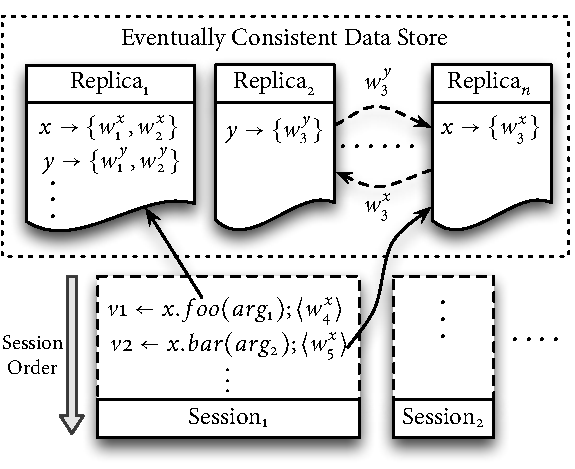
\includegraphics[width=0.75\columnwidth]{Figures/SystemModel}
\caption{Quelea system model.}
\label{fig:sysmod}
\end{figure}

Figure~\ref{fig:sysmod} provides a schematic diagram of our system model. The
distributed store is composed of a collection of \emph{replicas}, each of which
stores a set of \emph{objects} ($x,y,\ldots$). We assume that every object is
replicated at every replica in the store. The state of an object at any replica
is the set of all updates (\emph{effects}) performed on the object. For
example, the state of $x$ at replica 1 is the set composed of effects $w^x_1$
and $w^x_2$.

Each object is associated with a set of \emph{operations}. The clients interact
with the store by invoking operations on objects. The sequence of operations
invoked by a particular client on the store is called a \emph{session}. The
data store is typically accessed by a large number of clients (and hence
sessions) concurrently. Importantly, the clients are oblivious to which replica
an operation is applied to; the data store may choose to route the operation to
the closest replica for minimizing latency, or route it to a different replica
in order to balance the load in the system. For example, the operations
\emph{foo} and \emph{bar} invoked by the same session on the same object, might
end up being applied to different replicas because replica 1 (to which
\emph{foo} was applied) might be unreachable when the client invokes
\emph{bar}.

When \emph{foo} is invoked on a object $x$ with arguments \emph{arg}$_1$ at
replica 1, it simply \emph{reduces} over the current set of effects at that
replica on that object ($w^x_1$ and $w^x_2$), produces a result $v1$ that is
sent back to the client, and emits a \emph{single} new effect $w^x_4$ that is
appended to the state of $x$ at replica 1. Thus, every operation is evaluated
over a \emph{snapshot} of the state of the object on which it is invoked. In
this case, we say that the effect $w^x_4$ \emph{witnesses} $w^x_1$ and $w^x_2$.
Alternatively, $w^x_1$ and $w^x_2$ are \emph{visible} to $w^x_4$, written
logically as $\vis{w^x_1}{w^x_4} \wedge \vis{w^x_2}{w^x_4}$, where $\visZ$ is
the visibility relation between effects. Visibility is an irreflexive (an
operation cannot see its own effect) and asymmetric relation, and only relates
effects produced by operations on the same object. Executing a read-only
operation is similar except that no new effects are produced.

The effect added to a particular replica is asynchronously sent to other
replicas. We assume that \emph{eventually} an effect applied at one replica
will be merged into all other replicas. Two effects $w^x_4$ and $w^x_5$ that
arise from the same session are said to be in \emph{session order} (written
logically as $\so{w^x_4}{w^x_5}$). Session order is an irreflexive, transitive
relation. The effects $w^x_4$ and $w^x_5$ arising from operations applied to
the same object $x$ are said to be under the \emph{same object} relation,
written $\sameobj{w^x_4}{w^x_5}$. Finally, we can associate every effect with
the operation that generated the effect with the help of a relation $\operZ$.
In the current example, $\oper{w^x_4}{foo}$ and $\oper{w^x_5}{bar}$ hold. For
simplicity, we assume all operation names across all object types are distinct.

This model admits all the inconsistencies associated with eventual consistency.
The goal of this work is to identify the precise consistency level for each
operation such that application-level constraints are not violated. In the next
section, we will concretely describe the challenges associated with
constructing a consistent bank account on top of an eventually consistent data
store. Subsequently, we will illustrate how our contract and specification
language, armed with the primitive relations $\visZ$, $\soZ$, $\sameobjZ$ and
$\operZ$, mitigates these challenges.

\section{Motivation}
\label{sec:motivation}

Consider how we might implement a highly available bank account on top of an
eventually consistent data store, with the \emph{integrity} constraint that the
balance should never drop below 0. Let us assume that the bank account object
provides three operations: \cf{deposit}, \cf{withdraw} and \cf{getBalance},
with the assumption that the withdraw fails if the account has insufficient
balance. Our goal is to choose the correct consistency level for each of these
operations such that (1) the balance never drops below zero and (2) the
\cf{getBalance} operation never incorrectly returns a negative balance. To be
able to do this, we need to consider the anomalies that could arise under
eventual consistency.

\begin{figure}
\centering
\subfigure[Unsafe withdraw]{\label{fig:unsafeWithdrawAnomaly}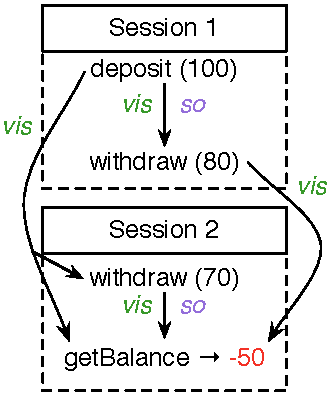
\includegraphics[width=0.34\columnwidth]{Figures/Motivation4}}
\hfill
\subfigure[Negative balance]{\label{fig:negativeBalanceAnomaly}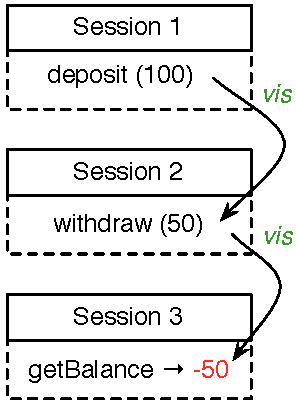
\includegraphics[width=0.31\columnwidth]{Figures/Motivation2}}
\hfill
\subfigure[Missing update]{\label{fig:missingUpdateAnomaly}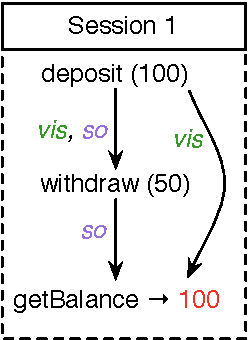
\includegraphics[width=0.26\columnwidth]{Figures/Motivation1}}
\caption{Anomalies possible under eventual consistency for the get balance operation.}
\label{fig:cleanliness_examples}
\end{figure}

Consider the execution shown in Figure~\ref{fig:unsafeWithdrawAnomaly}. Assume
that all operations in the figure are on the same bank account object with the
initial balance being zero. Session 1 performs a \cf{deposit} of 100, followed
by a \cf{withdraw} of 80 in the same session. The \cf{withdraw} operation
witnesses the deposit and succeeds\footnote{Although visibility and session
order relations relate effects, we have abused the notation in these examples
to relate operations, with the idea that the relations relate the effect
emitted by those operations}. Subsequently, session 2 perform a \cf{withdraw}
operation, but importantly, due to eventual consistency, only witnesses the
\cf{deposit} from session 1, but not the subsequent withdraw. Hence, this
\cf{withdraw} also \emph{incorrectly} succeeds, violating the integrity
constraint. A subsequent \cf{getBalance} operation, that happens to witness all
the previous operations,  would report a negative balance.

It is easy to see that the only way to ensure the integrity constraint on
\cf{balance} is to prevent concurrent withdrawals on the same bank account
object. This can be done by insisting that \cf{withdraw} be executed with
strong consistency properties. Although this prevents the integrity constraint
from being violated, a strongly consistent \cf{withdraw} itself is not
sufficient to prevent \cf{getBalance} from ever reporting a negative balance to
the end user.

Consider the execution shown in fig.~\ref{fig:negativeBalanceAnomaly}, which
consists of three concurrent sessions performing a \cf{deposit}, a
\cf{withdraw}, and a \cf{getBalance} operation, respectively, on the same bank
account object. As before, assume that the initial balance in the account is
zero. As the \cf{vis} edge indicates, operation \cf{withdraw(50)} in session 2,
can witnesses the effects of \cf{deposit(100)} from session 1, leading it to
rightfully conclude that the current balance is 50. Consequently,
\cf{withdraw(50)} is performed safely. The effect of this \cf{withdraw}
operation subsequently becomes visible to the \cf{getBalance} in Session 3.
However, because \cf{getBalance} only witnesses the effect of the \cf{withdraw}
operation from session 2, but not the \cf{deposit} from session 1, reports the
balance of negative 50 to the user.

Producing a negative balance is not the only inconsistency that the user is
exposed to under an eventually consistent bank account. Figure
~\ref{fig:missingUpdateAnomaly} shows an execution where the \cf{getBalance}
operation in a session does not witness the effects of an earlier \cf{withdraw}
operation performed in the same session, possibly because it was served by a
replica that has not yet merged the \cf{withdraw} effect, served by a different
replica. This anomaly leads the user to incorrectly conclude that the
\cf{withdraw} operation failed to go through.

Although it is easy to understand the reasons behind the occurrence of the
aforementioned negative balance and missing update anomalies, finding the
appropriate fixes is not readily apparent. Making \cf{getBalance} a strongly
consistent operation is definitely sufficient to avert anomalies, but is it
really necessary? Given the cost of enforcing strong
consistency~\cite{DynamoDB, Pileus}, it is preferable to avoid it unless
there are no viable alternatives.  Exploring the space of these alternatives
requires understanding the subtle differences in semantics of various kinds
of weak consistency alternatives.

\subsection{Specifications and Contracts}

\name helps facilitate the mapping of operations to appropriate consistency
levels by letting the programmer declare application-level consistency
constraints as \emph{contracts} that axiomatically specify the set of allowed
executions involving this operation.  In the case of the bank account example,
any execution that does not exhibit the anomalies described in the previous
section is a \emph{well-formed} execution on the bank account object.  By
specifying the set of legal executions for each data type in terms of a trace
of operation invocations on that type, \name\ ensures that all executions over
that type are well-formed.

In our running example, it is clear that in order to preserve the integrity
constraint, the \cf{withdraw} operation must be strongly consistent.  That is,
given two \cf{withdraw} operations $a$ and $b$, either $a$ is visible to $b$ or
vice versa. Utilizing the primitive relations described in
Section~\ref{sec:sysmod}, we express this application-level consistency
requirement as a contract or specification over \cf{withdraw}:
\vspace{-.5em}
\begin{smathpar}
\begin{array}{l}
\forall (a : \rcf{withdraw}).~\sameobj{a}{\cureff} \Rightarrow a = \cureff \vee \vis{a}{\cureff} \vee \vis{\cureff}{a}
\end{array}
\end{smathpar}
\noindent Here, $\cureff$ stands for the effect emitted by the \cf{withdraw} operation.
The syntax $a:\rcf{withdraw}$ states that $a$ is an effect which was emitted
by a \cf{withdraw} operation i.e., $\oper{a}{\rcf{withdraw}}$ holds.  The
contract specifies that if the current operation emits an effect $\cureff$,
then for any operation $a$ which was emitted by a \cf{withdraw} operation, it
is the case that $a = \cureff$ or $a$ is visible to $\cureff$, or vice versa.
Any execution on a bank account object that preserves the above contract for a
\cf{withdraw} operation is said to be derived from a correct implementation of
\cf{withdraw}.

\noindent For \cf{getBalance}, we construct the following contract:
\begin{smathpar}
\begin{array}{l}
\forall (a:\rcf{deposit}), (b:\rcf{withdraw}), (c: \rcf{deposit} \vee \rcf{withdraw}). \\
\qquad \vis{a}{b} \wedge \vis{b}{\cureff} \Rightarrow \vis{a}{\cureff} \\
\qquad \wedge~ (\soZ \cap \sameobjZ) (c,\cureff) \Rightarrow \vis{c}{\cureff}
\end{array}
\end{smathpar}
\noindent The expression $c:\rcf{deposit} \vee \rcf{withdraw}$ states that $c$ is an
effect that was emitted either by a \cf{deposit} or a \cf{withdraw} operation.
If a \cf{withdraw} $b$ is visible to \cf{getBalance}, then all \cf{deposit}
operations $a$ visible to the \cf{withdraw} should also be visible to
\cf{getBalance}. This prevents negative balance anomalies.

Our specification language provides operators to compose
relations. Thus, the syntax $(R_1 \cap R_2)(a,b)$ is equivalent to $R_1(a,b)
\wedge R_2(a,b)$. The last line of the above contract says that if a
\cf{deposit} or a \cf{withdraw} operation precedes a \cf{getBalance} operation in
session order, and is applied on the same object as the \cf{getBalance}
operation, then it must be the case that the \cf{getBalance} operation
witnesses the effects of the preceding operations.

Since there are no restrictions on when and how a \cf{deposit} operation can
execute, its contract is simply $\true$.

\subsection{From Contracts to Implementation}

Notice that the contracts for \cf{withdraw} and \cf{getBalance} only express
application-level consistency requirements, and make no reference to the
semantics of the underlying store. To write contracts, a programmer only needs
to reason about the semantics of the application under the \name system model.
The mapping of application-level consistency requirements to appropriate
store-level guarantees is done automatically behind-the-scene.

How might one go about ensuring that any execution adheres to the contract? The
challenge is that a contract provides a declarative (axiomatic) specification
of an execution, while what is required is is an operational procedure for
\emph{enforcing} its implicit constraints. One strategy would be to execute
operations speculatively.  Here, operations are tentatively applied as they are
received from the client or other replicas. We can maintain a runtime
manifestation of executions, and check well-formedness conditions at runtime,
rolling back executions if they are ill-formed. However, the overhead of state
maintenance and the complexity of user-defined contracts make this technique
infeasible in practice.

We devise a static approach instead. Contracts are analyzed with the help of a
theorem prover, and statically mapped to a particular store-level consistency
property that the prover guarantees preserves contract semantics. We call this
procedure \emph{contract classification}. Given the variety and complexity of
store level consistency properties, the idea is that the system implementor
parameterizes the classification procedure by describing the store semantics in
the \emph{same} contract language as the one used to express the contract on
the operations. In the next section, we describe the contract language in
detail and describe the classification procedure for a particular store
semantics.
